\chapter{Wavelets}
\label{ch:dwt}
In this chapter, we will introduce wavelet functions and the \emph{Discrete Wavelet Transform} (DWT).
The DWT allows us to transform our signal into a new basis in which it is sparse.
\begin{equation}
\bs x = \bs \Psi \bs w
\end{equation}
that takes the dense signal $\bs x$ and sends it into a domain in which its transformation $\bs w = \bs \Psi^T \bs x$ is sparse.

\section{Discrete Cosine Transform}
\emph{An aside on the DCT. Used in old JPEG standard (ref). Formulae. Interpretations. Pictures.}
However, before we discuss wavelets, we will briefly introduce the \emph{Discrete Cosine Transform} (DCT)

\section{Wavelet transforms}
\subsection{Haar wavelets}
Finding a set of basis functions $\bs\Psi$ that achieve such a transformation lies at the heart of many lossy compression techniques.
For instance, in image processing the JPEG 2000 standard is a widely used lossy compression technique that relies on this principle.
The original image $\bs x$ is transformed into $\bs w$ using the so-called \emph{Discrete Cosine Transform}.
The basis matrix $\bs \Psi$ is orthogonal, so $\bs x$ and $\bs w$ have the same $l_2$ norm.
In the original signal $\bs x$ the length is spread across many of its coefficients.
On the other hand, most of the length of $\bs w$ is concentrated in a few of its coefficients.
A large fraction of the entries in $\bs w$ are very close to zero. 
By deleting these entries in $\bs w$ and only storing the non-zero coefficients (and the corresponding basis functions), we can obtain a compressed version $\hat{\bs w}$. 
This allows us to significantly reduce the amount of data that needs to be stored without affecting the visual quality in the reconstructed image $\hat{\bs x} = \bs\Psi\hat{\bs w}$.

It is important to note here that the choice of basis functions $\bs \Psi$ typically has a significant effect on the performance of the reconstruction algorithms.

The simplest wavelet basis transformation is based on the Haar wavelets.
Figure \ref{fig:haarlenna} vizualises a basis transformation of the original image $\bs x$ to $\bs w$. 
This example uses a Haar wavelet basis at the first scale.
We will explain the Haar wavelet transformations of images and videos in more detail in the next chapter.
Dark areas correspond to small coefficients.
Note that most entries in $\bs w$ are near zero. 
In practice, we approximate these entries as zero and treat $\bs w$ as sparse.

\begin{figure}
\center
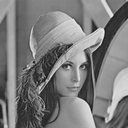
\includegraphics{Images/128.png}
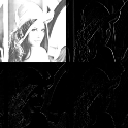
\includegraphics{Images/haar.png}
\caption{Original image $\bs x$ (left) and its Haar basis transformation $\bs w$ (right). See next chapter for more details on Haar wavelets.}
\label{fig:haarlenna}
\end{figure}

\subsection{Daubechies Wavelets}
\emph{Intuition. Where do the coeffs come from. Matrices. Boundary conditions.}


\section{Forming the basis matrix}
\emph{1D, 2D, 3D case. Different scales}

For a deeper introduction into wavelets see \cite{stollnitz1995}.
For more information on wavelet compression techniques, see \cite{devore1992}.

